% SandBlocks - Copyright 2024 Thiago M. de Oliveira. Solderpad Hardware License v2.1
% Script     : glossary.tex                                         Date: 2025.02.18
% Author     : Thiago M. de Oliveira <thiagomoraisee@gmail.com>
% Description: This annex chapter presents the acronyms and conventions used in this
%              Document.

\section{Glossary and conventions}
\label{sec:glossary_and_conventions}

The table \ref{tab:glossary} shows the acronyms and abbreviations used in this document.
\begin{table}[h]	
    \centering
	\rowcolors{2}{white}{sandblue!10}
    \begin{tabular}{|>{\centering\arraybackslash}p{1.5cm}|
                     >{\raggedright\arraybackslash}p{6.5cm}|}
		\arrayrulecolor{sandnavy!50}\hline
		\rowcolor{sandnavy!50}\hline
        % Columns labels:
        \textcolor{sandwhite}{\textbf{Term}}    &
        \textcolor{sandwhite}{\textbf{Meaning}} \\ \hline
        % Rows contents:
        FXRND & Fixed Point Rounder. The block's name.                                                     \\ \hline
        IWL   & Integer Wordlength. Used to specify the number of integer bits of a fixed point data.      \\ \hline
        LSB   & Least Significant Bit.                                                                     \\ \hline
        LSS   & Least Significant Sample.                                                                  \\ \hline
        MSB   & Most Significant Bit.                                                                      \\ \hline
        MSS   & Most Significant Sample.                                                                   \\ \hline
        N/A   & Not Applicable. Indicates that the referred info/section is not applicable to the context. \\ \hline
        PPA   & Power, Performance and Area.                                                               \\ \hline
        RND   & Round. Reffers to fixed-point quantization mode.                                           \\ \hline
        RTL   & Register Transfer Level.                                                                   \\ \hline
        SAT   & Saturation. Reffers to fixed-point overflow mode.                                          \\ \hline
        TBD   & To Be Done. Used to indicate that the feature/section will be implemented later.           \\ \hline
        WL    & Wordlength. Used to specify the number of bits of a data.                                  \\ \hline
	\end{tabular}
    \caption{Acronyms and abbreviations.}
    \label{tab:glossary}
\end{table}

\subsection{Fixed-point representation}
\label{sec:fixed_point_representation}

In some blocks, and behavioral explanations with fixed-point arithmetic there will be used the standard adopted by IEEE 1666-2023 SystemC to represent fixed-point data formats and arithmetic operations. This representation uses the pair $<WL, IWL>$ for representing a sugned/unsigned binary number with WL bits of wordlength and IWL integer bits. This representation gives a range of $\left[0, 2^{WL-IWL}-1 \right] / 2^{WL}$ for unsigned numbers and $\left[-2^{WL-IWL}, 2^{WL-IWL}-1 \right] / 2^{WL}$ for signed numbers. 

In some block representations, precision calculations and descriptions involving fixed-point arithmetic, the IEEE 1666-2023 SystemC standard will be used to represent fixed-point data formats and arithmetic operations. This standard defines a number using the pair $<WL, IWL>$, where WL represents the total word length (in bits) and IWL denotes the number of integer bits. The representation range for both signed and unsigned numbers is given by the equations \eqref{eq:range_unsigned} and \eqref{eq:range_signed} below:


\begin{equation}
    R_{unsigned} = \left[0, 2^{WL-IWL}-1 \right] / 2^{WL}
    \label{eq:range_unsigned}
\end{equation}

\begin{equation}
    R_{signed} = \left[-2^{WL-IWL},2^{WL-IWL}-1 \right] / 2^{WL}
    \label{eq:range_signed}
\end{equation}

This notation ensures a consistent and well-defined approach to handling fixed-point arithmetic across different blocks.

\subsection{Data representations}
\label{sec:data_representations}

Figure \ref{fig:data_connections} shows the color scheme for data representation, bit mapping, and data interconnections used throughout this document.

\begin{figure}[htb]
    \centering
    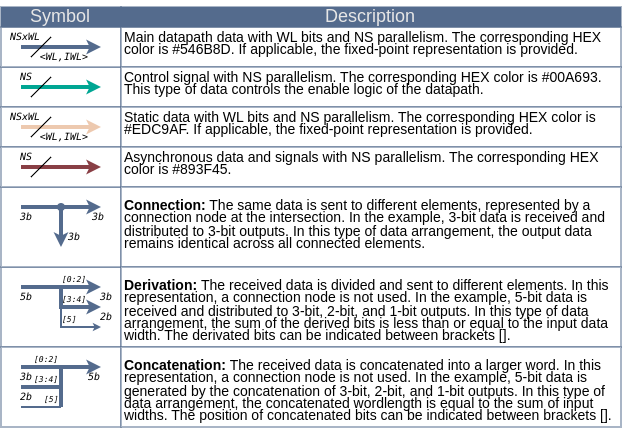
\includegraphics[width=9cm]{../../documentation/images/sandblocks_data_connections.png}
    \caption{Data representation and connections.}
    \label{fig:data_connections}
\end{figure}

